\documentclass[10pt]{article}
\usepackage{icmlko}

\icmlmeta{IP 파운데이션 월드모델}{191}{둘 다 되는 비율이 없다}{노트 190이 ``트리의 안쪽 곡면이 왜 평평한가''를 남겼다. 도메인 탈락이 아니었고, 행을 늘리면 트리가 나아지는데 그러면 능형이 무너진다}

\begin{document}

\twocolumn[
\icmlheader

\begin{abstract}
노트 190이 안쪽 시간 분할로 초매개변수를 고르는 규약을 세우면서 ``트리의
안쪽 곡면이 평평한 것이 \emph{행이 적어서}인지 \emph{도메인이 빠져서}인지
안 갈랐다''를 남겼다. 갈랐다. \textbf{도메인 탈락이 아니다} --- 안쪽 최소
행을 25에서 12로 낮춰 도메인을 일곱에서 아홉으로 되살려도(팝업은 여전히
못 들어온다) 트리의 봉우리 지수가 \textbf{0.198 에서 0.203} 으로 사실상
그대로다. 그러면 행인가. 학습 구간 안에서 앞쪽이 차지하는 비율을 0.50 ·
0.70 · 0.85 로 훑었다. \textbf{단순하지 않다} --- 트리의 봉우리 지수가
\textbf{0.301 · 0.203 · 0.378} 로 비단조이고, 능형은 \textbf{0.677 · 0.624
· 0.266} 으로 끝에서 무너진다. 두 힘이 맞서고 있다: \textbf{앞쪽을 늘리면
안쪽 학습행이 5,085 에서 8,708 로 늘어 트리의 용량이 제자리를 찾고}, 동시에
\textbf{안쪽 평가행이 5,206 에서 1,583 으로 줄어 점수가 시끄러워져 봉우리가
뭉개진다.} 트리는 앞의 힘이 크고 능형은 뒤의 힘이 크다. 그래서
\textbf{둘 다 문턱 0.5 를 넘는 비율이 없다} --- 0.85 에서 트리가 제일 높지만
(0.378) 여전히 아래이고 거기서 능형이 0.266 으로 무너진다. \textbf{현행
0.70 을 유지한다} --- 능형 셋은 조정되고(0.624) 트리는 가드에 막힌다(0.203).
곁가지로 하나: \textbf{봉우리 지수가 진단으로 제대로 작동한다.} 평가행이
1,583 으로 줄자 능형의 지수가 0.624 에서 0.266 으로 떨어졌다 --- 지표가
``신호 대 잡음''을 재고 있다는 뜻이고, 그것이 이 지표를 만든 이유다.
\textbf{결론은 부정형이다} --- 챔피언은 이 자료로는 조정할 수 없다. 고칠 수
있는 설정 문제가 아니라 표본이 모자란 것이다.
\end{abstract}
]

\begin{figure*}[t]
\centering
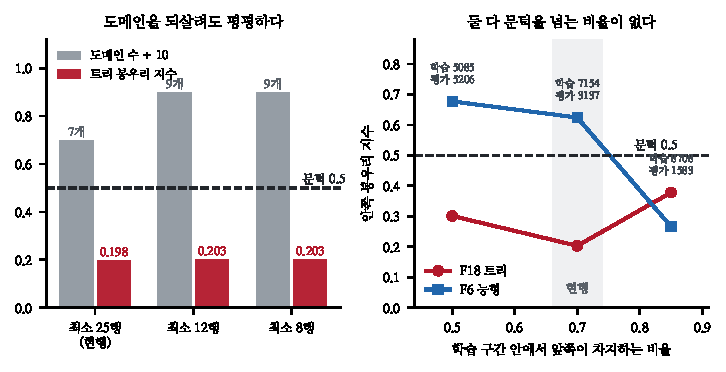
\includegraphics[width=.72\textwidth]{figs/frac.pdf}
\caption{왼쪽 --- 도메인을 되살려도 평평하다. 오른쪽 --- 둘 다 문턱을 넘는
비율이 없다.}
\end{figure*}

\section{도메인 탈락이 아니다}

\begin{table}[t]
\centering\tsize
\caption{안쪽 최소 행을 낮춰 도메인을 되살린다.}
\begin{tabular}{lrrr}
\toprule
& 도메인 & 트리 봉우리 & \\
\midrule
최소 25행 (현행) & 7 & 0.198 & \\
최소 12행 & 9 & \textbf{0.203} & 도서·아이돌 복귀 \\
최소 8행 & 9 & 0.203 & 더 안 는다 \\
\bottomrule
\end{tabular}
\end{table}

\claimx{\textbf{도서와 아이돌을 되살려도 0.005 움직인다.} 팝업은 어느
문턱에서도 안 들어온다 --- 2025년 이전 행이 열여섯뿐이다(노트 132).}{그러니
노트 190에서 적은 ``도메인 셋이 빠져서일 수 있다''는 읽기는 \textbf{반증
됐다.} 그 노트에서 ``자료로는 못 가른다''고 적어 뒀는데, 갈렸다.}

\section{행도 단순하지 않다}

\begin{table}[t]
\centering\tsize
\caption{학습 구간 안에서 앞쪽 비율을 바꾼다.}
\begin{tabular}{lrrrr}
\toprule
비율 & 학습행 & 평가행 & 트리 & 능형 \\
\midrule
0.50 & 5{,}085 & 5{,}206 & 0.301 & \textbf{0.677} \\
0.70 & 7{,}154 & 3{,}137 & 0.203 & \textbf{0.624} \\
0.85 & 8{,}708 & 1{,}583 & \textbf{0.378} & 0.266 \\
\bottomrule
\end{tabular}
\end{table}

\claimx{\textbf{두 힘이 맞선다.} 앞쪽을 늘리면 안쪽 학습행이 5,085 에서
8,708 로 늘어 트리의 용량이 제자리를 찾고, 동시에 안쪽 평가행이 5,206 에서
1,583 으로 줄어 점수가 시끄러워진다.}{트리는 앞의 힘이 크고(0.301$\to$0.378)
능형은 뒤의 힘이 크다(0.677$\to$0.266). \textbf{같은 손잡이가 두 형태에
반대로 작용한다.}}

\claimx{\textbf{둘 다 문턱을 넘는 비율이 없다.} 0.85 에서 트리가 제일
높지만(0.378) 여전히 아래이고, 거기서 능형이 무너진다(0.266).}{\textbf{현행
0.70 을 유지한다} --- 능형 셋이 조정되고(0.624) 트리는 가드에 막힌다(0.203).
셋을 얻고 하나를 지키는 쪽이 낫다.}

\section{지표가 제대로 작동한다}

\claimx{\textbf{평가행이 1,583 으로 줄자 능형의 봉우리가 0.624 에서 0.266
으로 떨어졌다.} 능형의 \emph{진짜} 최적 알파가 바뀐 것이 아니라 그것을
\emph{보는 눈}이 흐려진 것이다.}{\textbf{봉우리 지수가 신호 대 잡음을 재고
있다는 확인이다} --- 그게 이 지표를 만든 이유다(노트 190). 노이즈를 늘리면
지수가 떨어져야 하고, 떨어졌다.}

\claimx{\textbf{그래서 결론이 부정형이다.} 챔피언 F18 은 이 자료로는 조정할
수 없다 --- 고칠 수 있는 설정 문제가 아니라 표본이 모자란 것이다.}{판을
올릴 여지가 없다는 말은 아니다. \textbf{안쪽 없이 조정하는 길}이 남아 있다
--- 예컨대 이론적으로 정한 값이나 다른 자료에서 옮겨 온 값. 다만 이
실험실은 그것을 검증할 방법이 없다.}

\begin{table}[t]
\centering\tsize
\caption{이 흐름의 조정 결과.}
\begin{tabular}{lrl}
\toprule
& 이득 & \\
\midrule
F6 능형 & $+$.0109 & 채택 ($t{=}4.51$) \\
F10 도메인별 & $+$.0125 & 채택 ($t{=}1.80$) \\
F11 합집합 & $+$.0130 & 채택 ($t{=}4.06$) \\
\textbf{F18 배깅} & \textbf{---} & \textbf{가드가 막음} \\
\bottomrule
\end{tabular}
\end{table}

\begin{table}[t]
\centering\tsize
\caption{남은 것.}
\begin{tabular}{ll}
\toprule
\textbf{팝업} & 어느 문턱에서도 안쪽에 못 들어온다 \\
반복 분할 & 한 번 자르지 말고 여러 번 잘라 평균 \\
문턱 0.5 & 여전히 네 점 사이에 그은 값 \\
\bottomrule
\end{tabular}
\end{table}

두 번째 줄이 제일 값이 크고 곧바로 할 수 있다. 지금은 학습 구간을 \emph{한
번} 잘라 안쪽 점수를 내는데, 그 점수 자체가 한 번 뽑기라 잡음이 크다 ---
비율 0.85 에서 능형이 무너진 것이 바로 그 잡음이다. \textbf{여러 시점에서
잘라 평균하면 봉우리 지수가 올라가야 하고, 그러면 트리도 문턱을 넘을 수
있다.} 넘으면 챔피언을 조정할 수 있고, 안 넘으면 ``표본이 모자란다''가
확정된다.

\end{document}
